\forceindent The observation of the first multiply-imaged, gravitationally lensed supernova (SN) in 2014, SN ``Refsdal", 
was a critical step forward for the SN cosmology community (Figure 1; \citet{Kelly:2015a}). As light from a distant
source passes through a gravitational lens, each subsequent image will appear to the observer delayed relative to the 
unlensed travel time. If the lensing potential is well known, then the {\bf time delay measurement  provides a direct constraint on
the Hubble constant that is completely independent of the local distance ladder.} There are certain degeneracies associated with
obtaining these constraints directly from time delays, which are broken in the case of a Type 1a ``standard candle" SN \citep{Kolatt:1998}. The very 
first multiply-imaged Type 1a SN (iPTF16geu) was discovered by \citet{Goobar:2016}, but attempts to constrain the time delays have been 
only moderately successful citing the need for a comprehensive mechanism that includes microlensing effects as a primary source of uncertainty 
\citep{More:2016}. We propose to perform a complete reanalysis of SN Refsdal in order to refine our constraints on the lensing parameters 
and define a rigorous methodology for use in the case of SN iPTF16geu and future lensed SNe. We will improve upon previous work by 
making substantial improvements to the photometry, and including the significant yet previously ignored effects of microlensing. 
Additionally, we will produce an open-source software package in the course of this work, optimized specifically for multiply-imaged SNe. 

\begin{figure}[h]
\centering
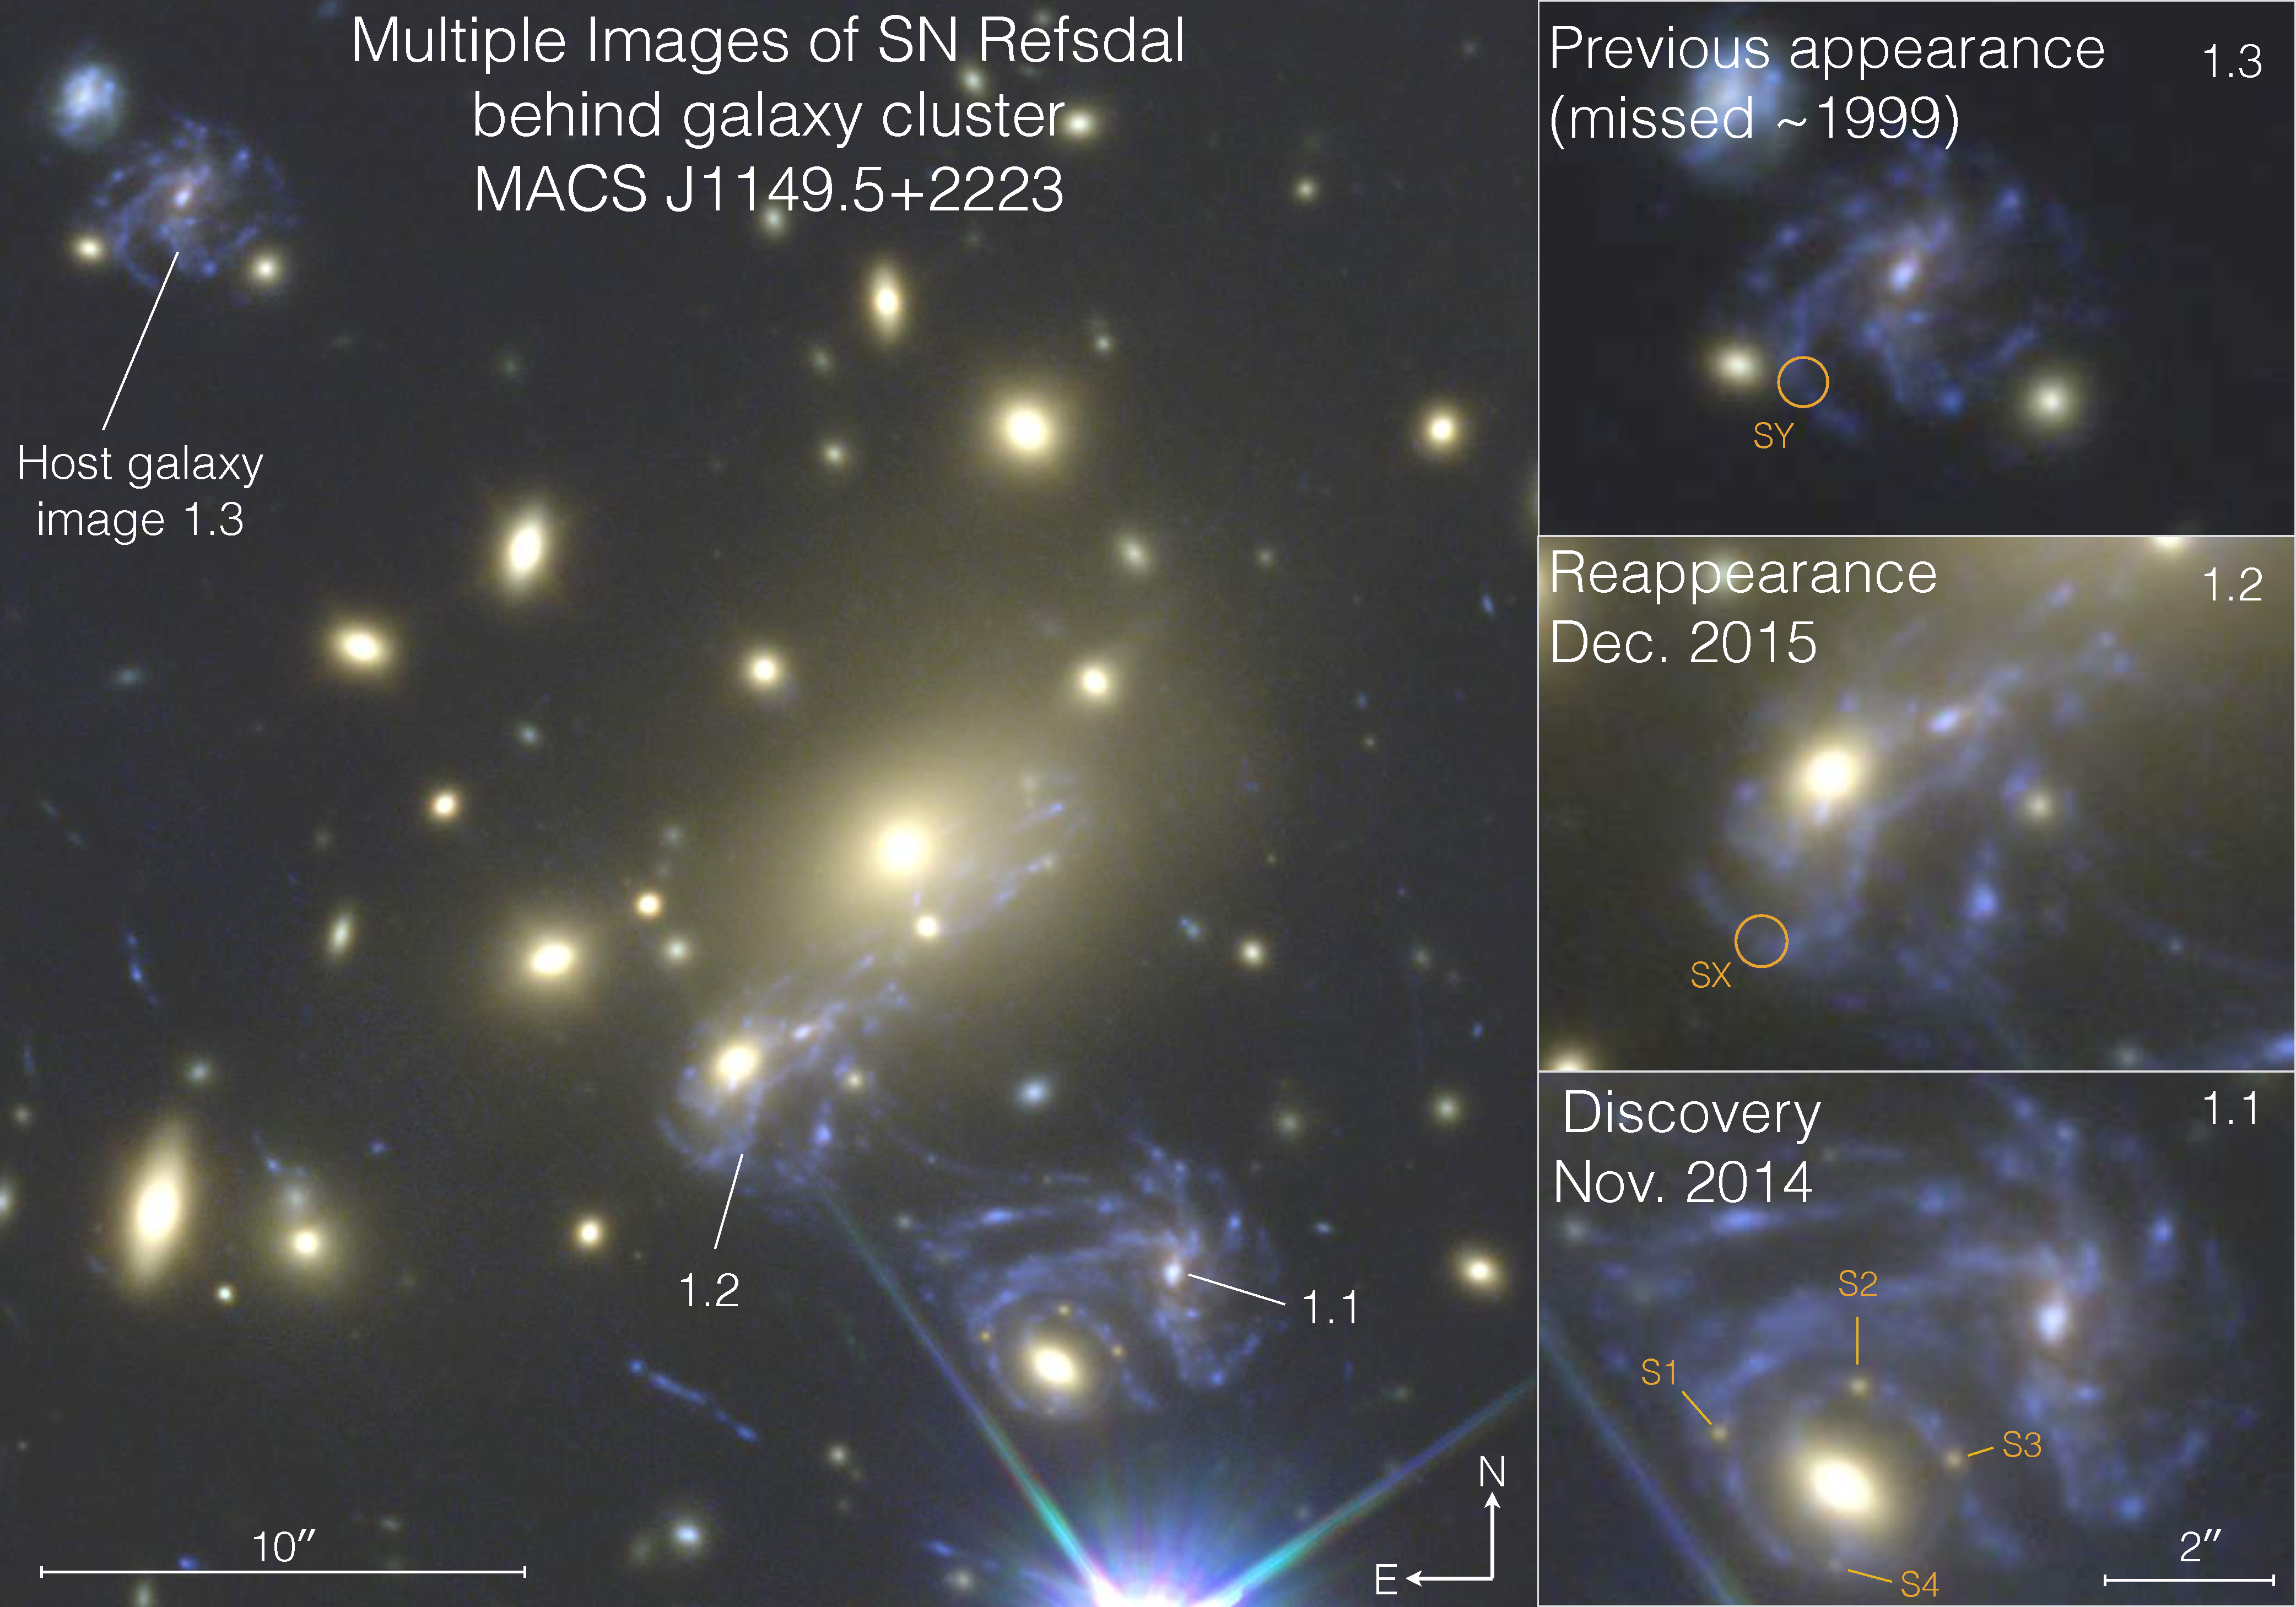
\includegraphics[width=0.75\textwidth]{FIG/refsdal_rodney.pdf}
\caption{
MACS J1149.6+2223 field, showing the positions of the three primary
images of the SN Refsdal host galaxy (labeled 1.1, 1.2, and 1.3). SN
Refsdal appears as four point sources in an Einstein Cross
configuration in the southeast spiral arm of image 1.1 \citep{Rodney:2016}}
\end{figure}

As a previously ignored check against systematic biases, our reanalysis will use both the \textit{PythonPhot} and the \textit{DOLPHOT} packages to 
perform photometric measurements. We will also measure the photometry in single-exposure images, allowing us to check for any deviations 
at very short timescales, indicative of very rapid microlensing events. \cite{Rodney:2016} measured flux using a single empirical 
point-spread function (PSF) fixed in time, derived from standard stars. However, as we know that the HST PSF does undergo 
subtle variations due to telescope ``breathing" (\textbf{CITE}), our re-analysis will use foreground stars within the MACS1149 imaging 
datasets to define a variable PSF model. \textbf{The reduction of systematic biases in the photometry and our improvements to the 
PSF will provide drastically ameliorated flux calculations, which in turn will increase the accuracy and precision of time delay measurements.}

Microlensing refers to small-scale gravitational lensing
perturbations due to massive objects along the light path of any one image of a
multiply-imaged SN. The effect of microlensing is to cause distortions in the SN light
curves that significantly limit the precision that can be achieved in the measurement of 
their time delays \citep{Dobler:2006}. Despite noting this significant source of uncertainty, the analyses performed for SN Refsdal and SN iPTF16geu 
have completely ignored microlensing due to its complexity (\cite{More:2016,Rodney:2016}). In preparing this proposal, we have already 
used flexible functions to preliminarily measure the effects of the type 1 microlensing on SN Refsdal (Figure 2), and it's 
\textbf{clear that microlensing must be taken into account} in order to ensure accurate time delay and magnification measurements. 
Therefore, we will \textbf{fully analyze the effects of microlensing on a multiply-imaged SN for the first time} and ensure they can be accurately
accounted for in future SN analysis.

\textbf{The next decade is expected to yield observations
of over 100 lensed SNe} that will require analysis \citep{Oguri:2010},
yet \textbf{there is no public software package for analyzing multiply-imaged SNe.}
In the course of this work, we are producing an open-source software package written 
in Python for use in this and future SN analysis. Specifically, efforts to measure the time 
delays of SN iPTF16geu, critical to a new measurement of $H_0$, have not been 
successful beyond broad constraints (\cite{Goobar:2016}, \cite{More:2016}). This new tool,
developed and tested in the course of reanalyzing SN Refsdal, will be used to make a time 
delay measurement in parallel to the Goobar et al. team when they make follow-up observations
later this year, providing an important independent check of such a measurement for the first time. 

\cite{Goobar:2016} concluded that the \textbf{rate of strongly lensed Type 1a SNe is likely much higher than
previously thought}, with implications for our constraints on $H_0$, the study of galaxy sub-structures,
and tests of theories of modified gravity. If the number of lensed Type 1a SNe observed in the JWST/LSST
era follows these predictions, then it will be absolutely essential to have a publicly available, standardized 
tool in place to accurately produce time delay and magnification measurements. The reanalysis of SN 
Refsdal offers a \textbf{unique chance} to develop the software and methodology necessary in the coming years for
analyzing new SNe \textbf{to obtain exciting scientific results}, including constraints on dark energy parameters and a
direct probe of the expansion rate of the universe, $H_0$.

\begin{figure}
\centering
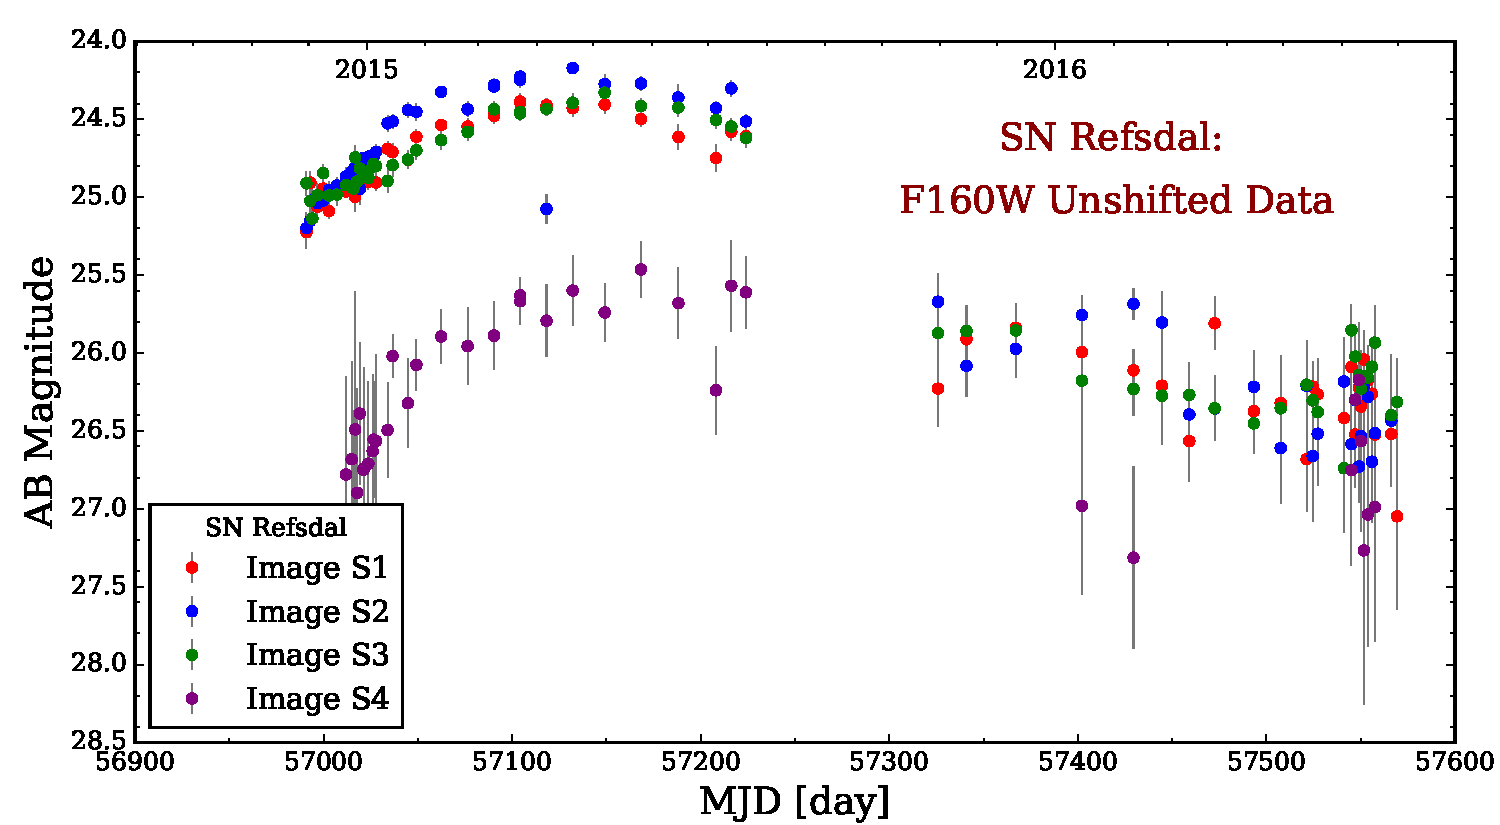
\includegraphics[width=.7\textwidth]{FIG/points_plot_2017.pdf}
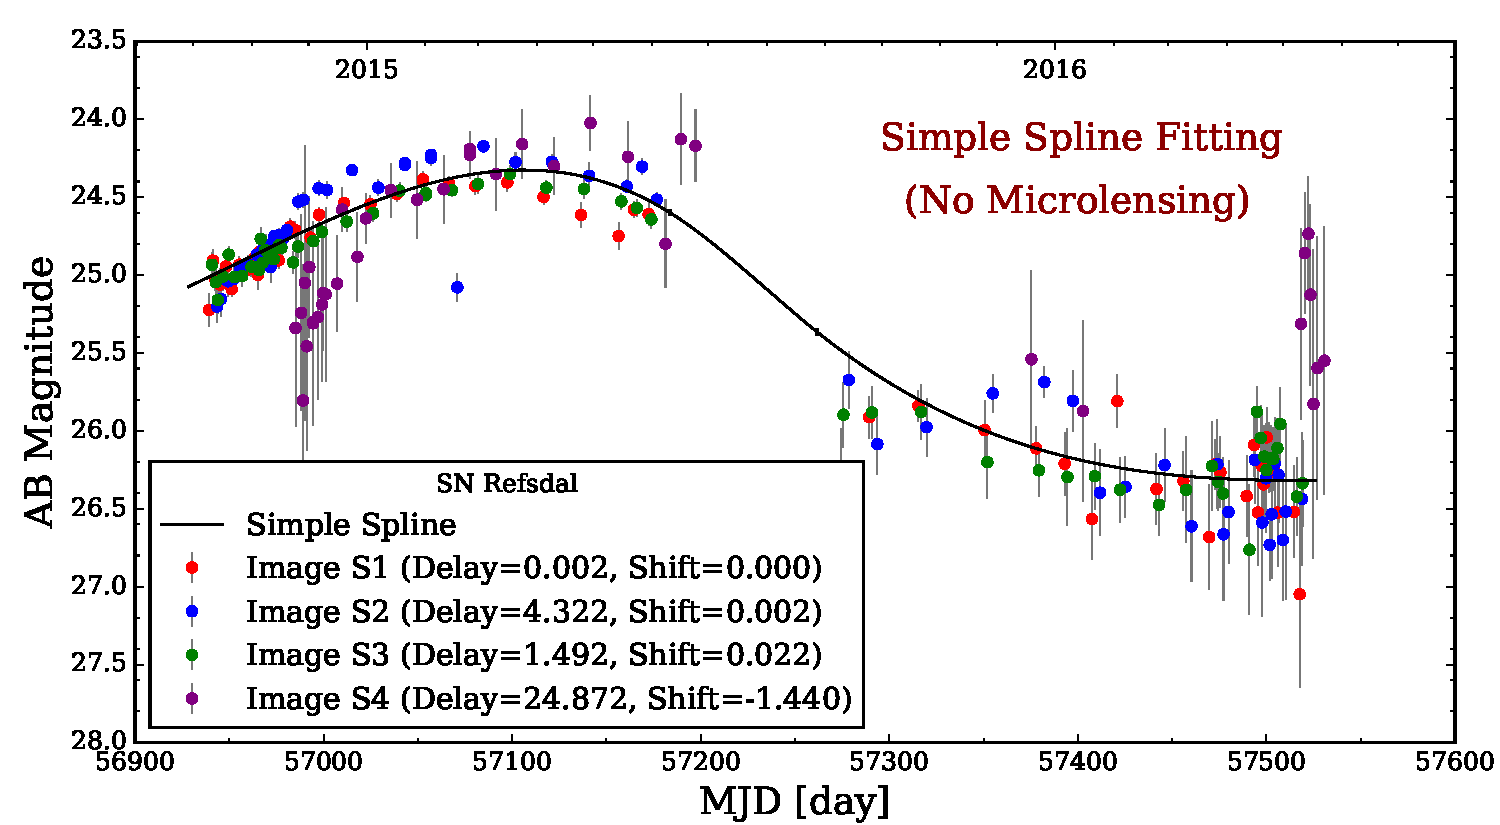
\includegraphics[width=.7\textwidth]{FIG/refs_plot_2017.pdf}
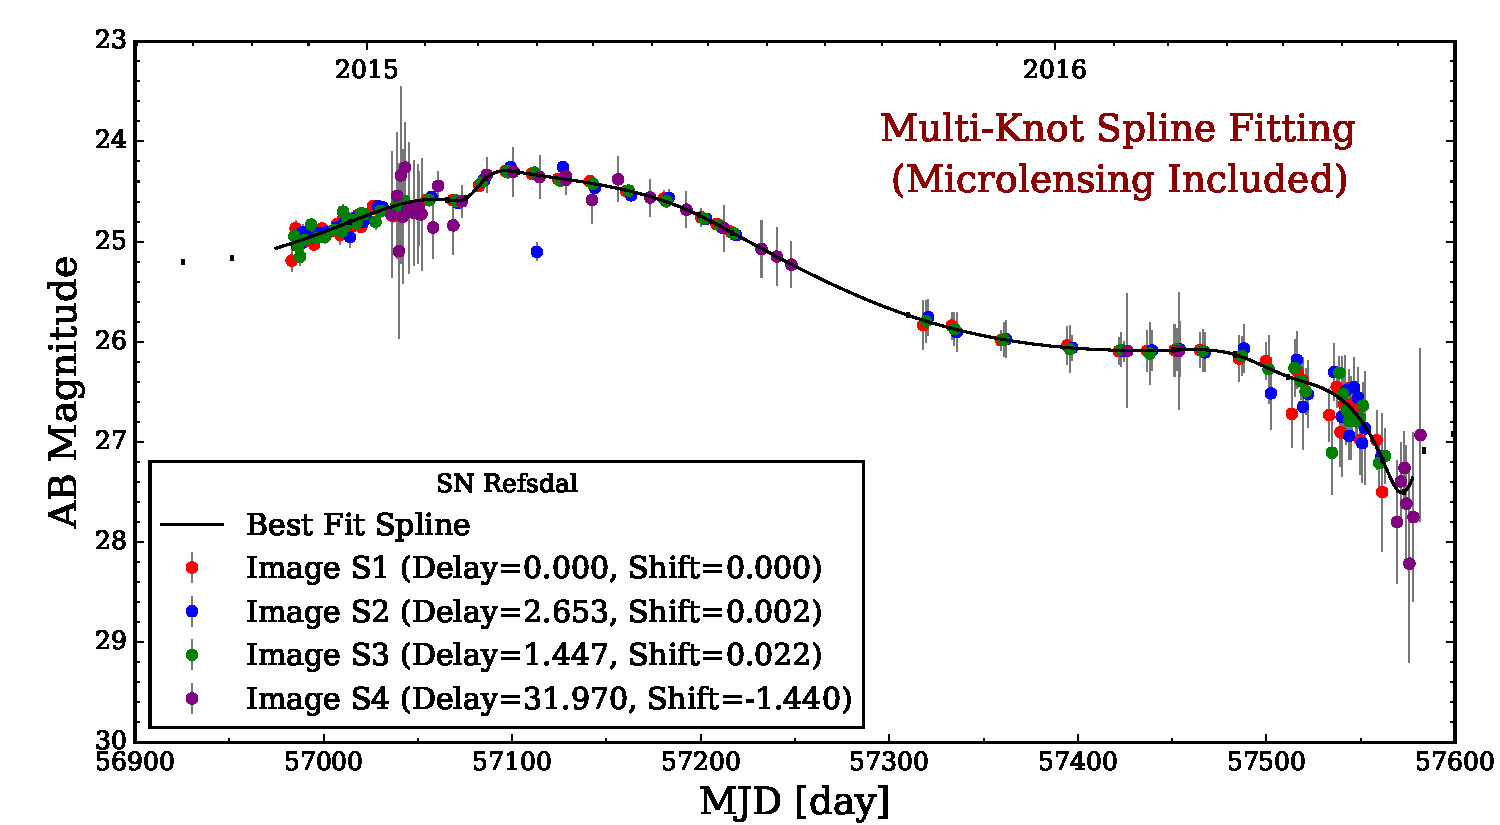
\includegraphics[width=.7\textwidth]{FIG/spline_plot_2017.pdf}
\caption{(Top) HST F160W data representing the four images of SN
Refsdal (Figure 1), with no lensing or time shifts. (Middle) Method of
fitting the SN Refsdal light curves from Rodney et al. 2016, which did
not consider microlensing effects. (Bottom) Preliminary results from 
this work using a multi-knot spline to fit the data. This method 
includes microlensing effects, which leads to a slight adjustment in 
time delay measurements. }
\end{figure}

\bigskip
 
 




